\begin{figure}
  \centering 
  \begin{subfigure}[b]{0.45\textwidth}
    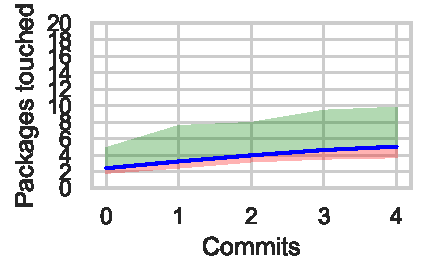
\includegraphics[width=\textwidth]{sections/results/packages/time_series_components_touched.packages.all.founders.commits_5.pdf}
    \caption{Packages for All founders (n=64, $\mu$=4.92, median=3.0 \& std=3.82)}
    \label{subfig:sections/results/packages/time_series_components_touched_packages_all_founders_commits_5_pdf}
  \end{subfigure}
  \begin{subfigure}[b]{0.45\textwidth}
    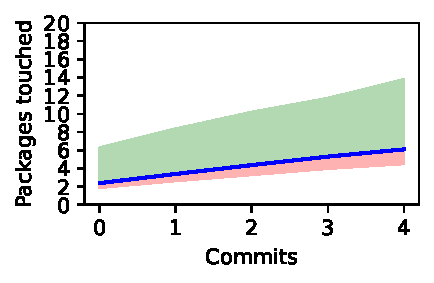
\includegraphics[width=\textwidth]{sections/results/packages/time_series_components_touched.packages.all.joiners.commits_5.pdf}
    \caption{Packages for All joiners (n=1277, $\mu$=6.09, median=3.0 \& std=4.66)}
    \label{subfig:sections/results/packages/time_series_components_touched_packages_all_joiners_commits_5_pdf}
  \end{subfigure}
\newpage 
\vspace{3mm}
  \begin{subfigure}[b]{0.45\textwidth}
    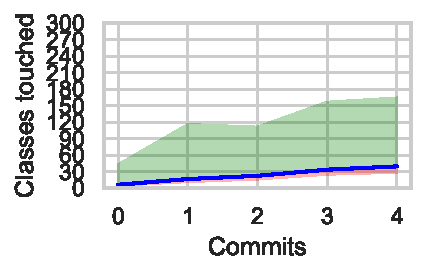
\includegraphics[width=\textwidth]{sections/results/classes/time_series_components_touched.classes.all.founders.commits_5.pdf}
    \caption{Classes for All founders (n=64, $\mu$=39.38, median=7.0 \& std=57.9)}
    \label{subfig:sections/results/classes/time_series_components_touched_classes_all_founders_commits_5_pdf}
  \end{subfigure}
  \begin{subfigure}[b]{0.45\textwidth}
    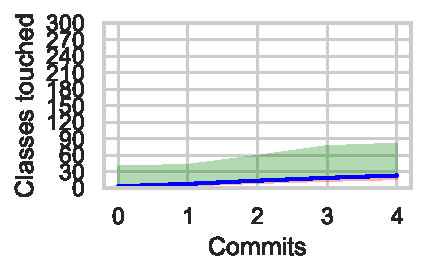
\includegraphics[width=\textwidth]{sections/results/classes/time_series_components_touched.classes.all.joiners.commits_5.pdf}
    \caption{Classes for All joiners (n=1277, $\mu$=22.77, median=6.0 \& std=28.25)}
    \label{subfig:sections/results/classes/time_series_components_touched_classes_all_joiners_commits_5_pdf}
  \end{subfigure}
\newpage 
\vspace{3mm}
  \begin{subfigure}[b]{0.45\textwidth}
    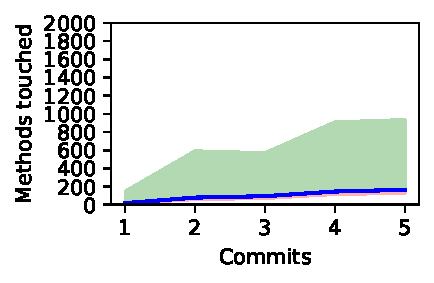
\includegraphics[width=\textwidth]{sections/results/methods/time_series_components_touched.methods.all.founders.commits_5.pdf}
    \caption{Methods for All founders (n=64, $\mu$=166.56, median=15.0 \& std=332.48)}
    \label{subfig:sections/results/methods/time_series_components_touched_methods_all_founders_commits_5_pdf}
  \end{subfigure}
  \begin{subfigure}[b]{0.45\textwidth}
    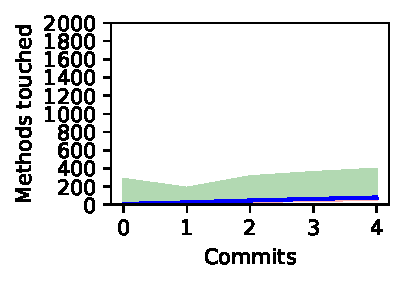
\includegraphics[width=\textwidth]{sections/results/methods/time_series_components_touched.methods.all.joiners.commits_5.pdf}
    \caption{Methods for All joiners (n=1277, $\mu$=80.35, median=12.0 \& std=138.17)}
    \label{subfig:sections/results/methods/time_series_components_touched_methods_all_joiners_commits_5_pdf}
  \end{subfigure}
\caption[Time Series for all compenents unit:commits category:6 commits:5]{A time series for the five (5) commits, excluding transient, with the average mean (blue line), all components touched (y-axis) against the number of commits (x-axis) for six (6) developer categories. Green is the standard deviation above the mean, and pink is the standard deviation below the mean.} 
    \label{fig:0_codebase_graph_latex_repository_graph_component_time_series_time_series_components_touchedmethods5_5}
\end{figure}
\clearpage 
\newpage 
